\documentclass[tikz,border=7pt]{standalone}
\usepackage{amsmath}
\usetikzlibrary{arrows.meta,positioning,fit}
\begin{document}
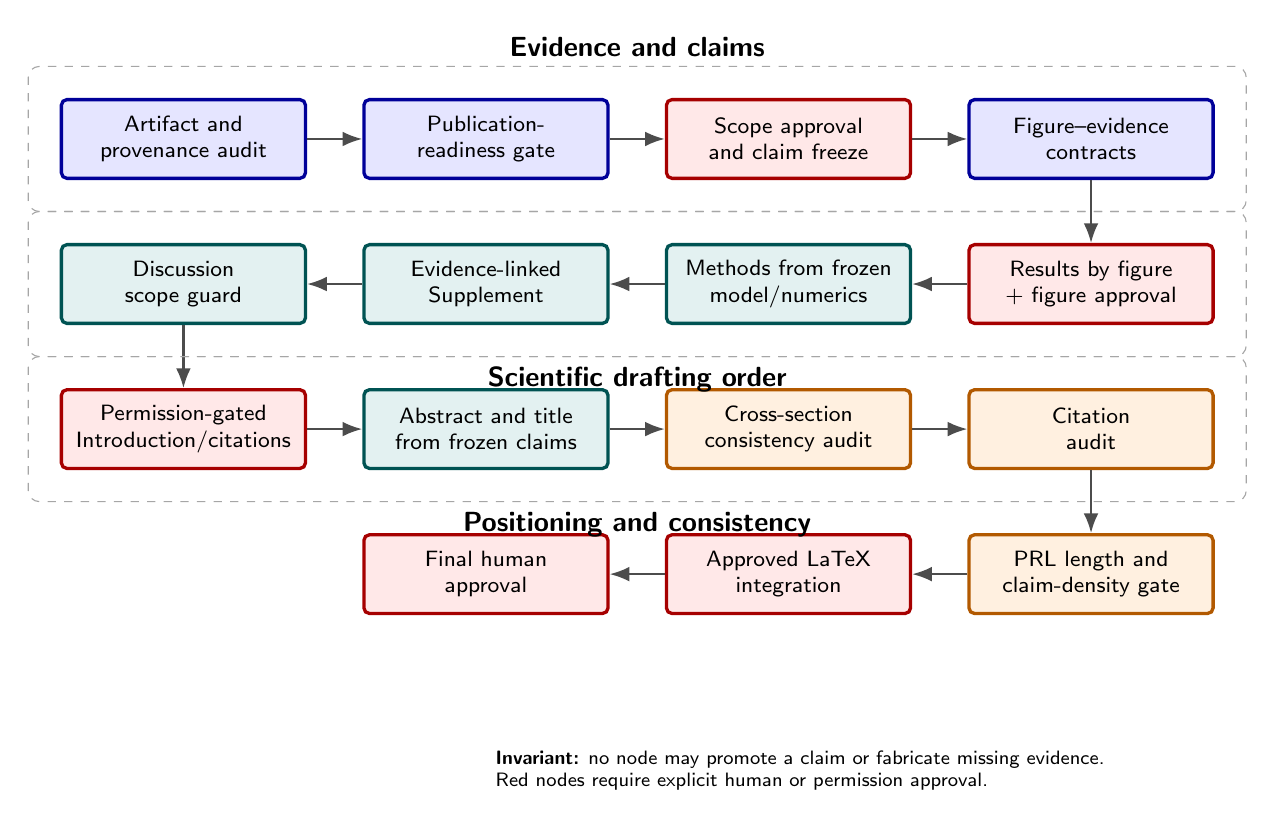
\begin{tikzpicture}[
  font=\sffamily\footnotesize,
  node distance=8mm and 7mm,
  box/.style={draw,rounded corners=2pt,minimum width=31mm,minimum height=10mm,align=center,very thick},
  evidence/.style={box,fill=blue!10,draw=blue!60!black},
  draft/.style={box,fill=teal!11,draw=teal!65!black},
  audit/.style={box,fill=orange!12,draw=orange!70!black},
  gate/.style={box,fill=red!9,draw=red!65!black},
  arrow/.style={-{Latex[length=2.5mm]},thick,draw=black!70}
]
\node[evidence] (artifact) {Artifact and\\provenance audit};
\node[evidence,right=of artifact] (ready) {Publication-\\readiness gate};
\node[gate,right=of ready] (claim) {Scope approval\\and claim freeze};
\node[evidence,right=of claim] (figcontract) {Figure--evidence\\contracts};

\node[gate,below=of figcontract] (results) {Results by figure\\+ figure approval};
\node[draft,left=of results] (methods) {Methods from frozen\\model/numerics};
\node[draft,left=of methods] (supplement) {Evidence-linked\\Supplement};
\node[draft,left=of supplement] (discussion) {Discussion\\scope guard};

\node[gate,below=of discussion] (intro) {Permission-gated\\Introduction/citations};
\node[draft,right=of intro] (abstract) {Abstract and title\\from frozen claims};
\node[audit,right=of abstract] (consistency) {Cross-section\\consistency audit};
\node[audit,right=of consistency] (citation) {Citation\\audit};

\node[audit,below=of citation] (length) {PRL length and\\claim-density gate};
\node[gate,left=of length] (latex) {Approved LaTeX\\integration};
\node[gate,left=of latex] (human) {Final human\\approval};

\draw[arrow] (artifact) -- (ready);
\draw[arrow] (ready) -- (claim);
\draw[arrow] (claim) -- (figcontract);
\draw[arrow] (figcontract) -- (results);
\draw[arrow] (results) -- (methods);
\draw[arrow] (methods) -- (supplement);
\draw[arrow] (supplement) -- (discussion);
\draw[arrow] (discussion) -- (intro);
\draw[arrow] (intro) -- (abstract);
\draw[arrow] (abstract) -- (consistency);
\draw[arrow] (consistency) -- (citation);
\draw[arrow] (citation) -- (length);
\draw[arrow] (length) -- (latex);
\draw[arrow] (latex) -- (human);

\node[draw=black!35,dashed,rounded corners,fit=(artifact)(figcontract),inner sep=4mm,label={[font=\bfseries\sffamily]above:Evidence and claims}] {};
\node[draw=black!35,dashed,rounded corners,fit=(results)(discussion),inner sep=4mm,label={[font=\bfseries\sffamily]below:Scientific drafting order}] {};
\node[draw=black!35,dashed,rounded corners,fit=(intro)(citation),inner sep=4mm,label={[font=\bfseries\sffamily]below:Positioning and consistency}] {};

\node[align=left,below=16mm of human,anchor=north west,font=\sffamily\scriptsize] (legend) {\textbf{Invariant:} no node may promote a claim or fabricate missing evidence.\\
Red nodes require explicit human or permission approval.};
\end{tikzpicture}
\end{document}
